\section{Development process and implementation}
\label{chap:development_process}

This chapter details the steps used during the development of the program. Features of the program were added iteratively, beginning with simply getting the LEDs to light up and then evolving to more sophisticated funcionality. The first iteration of the code simply turned on the LEDs. After this, an opening sequence was added to the program, the details of which and why it was added is explained more in section \ref{subsec:dev_pros_opening_seq}. Afterwards, a polling technique was used to test the buttons on the game pad. With the correct flags set a number will be written to a specific location in memory which indicates what buttons are being pressed. This number is then shifted eight places to the left to comply with the way LEDs are lightened up.

The next step was to make interrupts work. A main function was constructed to set the correct flags. When these are set the device goes to sleep and waits for an interrupt. A main focus was to abort the interrupts as quickly as possible. More on this in section \ref{subsec:dev_pros_interrupts}.

\subsection{Pre-assignment setup}
\label{subsec:pre-assingment_setup}

The assignment involves a lot of GPIO usage, and therefore some values are used over and over. The register design is set up so that three registers are storing GPIO constants and one register is used for simulating a wait for the opening sequence. They each have an alias to be easier to access. GPIO\_PA\_BASE was renamed gpio\_o and GPIO\_PC\_BASE was renamed to gpio\_i, GPIO\_BASE was renamed gpio. The remaining registers from r0 to r7 is used for variable content. See table \ref{tab:register_design} in appendix A on page \pageref{tab:register_design} for an overview of the registers.

\subsection{Sound synthesis}
The three sound effects we've implemented are all generated in real-time on the board.
We made three different sound effects: a coin blip, a laser, and a level-up sound.
They are all based on a simple waveform, either a square wave or a sawtooth.
Each sound has parameters that are allowed to change for each playback.
Those parameters include frequency, slide, and ADSR parameters.

\subsubsection{ADSR}

A waveform with constant frequency alone would not provide the sound effects we wanted. We therefore implemented a ADSR envelope \cite{adsr}.
The envelope consists of an attack period, a decay period, a sustain level and a release period, as seen in figure \ref{fig:adsr}.

\begin{itemize}
    \item The attack periode is the time to use from zero to maximum amplitude.
    \item The decay is the time from max amplitude down to the sustain level.
    \item The sustain level is the amplitude to rest on between the decay and release periods.
    \item The release indicates how much time to spend fading from the sustain level to zero volume.
\end{itemize}

\begin{figure}[ht!]
    \begin{center}
    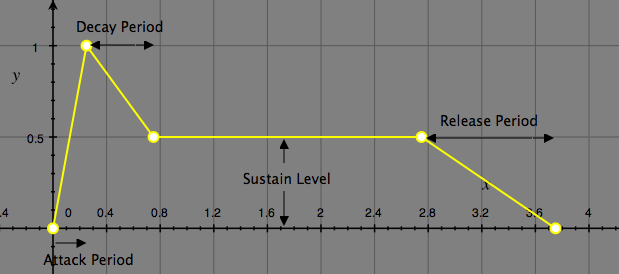
\includegraphics[width=0.8\textwidth]{assets/img/adsr.png}
    \caption{A ADSR envelope}
    \label{fig:adsr_envelope}
    \end{center}
\end{figure}

\subsection{Pre-recorded melody}

For the start-up melody, we chose to produce a song using FL Studio, a digital audio workstation. We would then export the .wav file and convert it to a C array, as a wav file consists of two channels of typically 44,100 samples per second, and $2^x$ bits per sample. Doing this, we could . We had to first export the song to a 16 bit int .wav file, as FL Studio didn't accept 8 bit int .wav. We opened the song in Audacity, as this audio editor allowed us to export it to a 8 bit int .wav file. Moreover, we used a Python library to convert the .wav samples to a C array, tailoring this general Python .wav interpreter code \cite{wav} to fit our needs. Our edited Python code to produce the C file that holds the two arrays that represents the two channels is shown below:

\begin{code}
import wave, struct

def pcm_channels(wave_file):
    stream = wave.open(wave_file,"rb")

    num_channels = stream.getnchannels()
    sample_rate = stream.getframerate()
    sample_width = stream.getsampwidth()
    num_frames = stream.getnframes()

    raw_data = stream.readframes( num_frames )
    stream.close()

    total_samples = num_frames * num_channels

    if sample_width == 1: 
        fmt = "%iB" % total_samples
    elif sample_width == 2:
        fmt = "%ih" % total_samples
    else:
        raise ValueError("Only supports 8 and 16 bit audio formats.")

    integer_data = struct.unpack(fmt, raw_data)
    del raw_data

    channels = [ [] for time in range(num_channels) ]

    for index, value in enumerate(integer_data):
        bucket = index % num_channels
        channels[bucket].append(value)

    return channels

f = open('song.c', 'w')

chan0, chan1 = pcm_channels('file.wav')[0], pcm_channels('file.wav')[1]

#Outputs the C code with the two arrays
f.write('#include <stdint.h>\n\nconst uint8_t channel0[] = {' + str(chan0)[1:-1]\
 + '};\n\nconst uint8_t channel1[] = {' + str(chan1)[1:-1] + '};')

\end{code}

\newpage

The sound clip lasted around 15 seconds, which results in $44100 samples/seconds * 15 seconds = 661500 samples$. 
Since this file was too large for the DAC, we shortened the song to 8 seconds, or 3.5 MB, which was small enough for the DAC to interpret.


\subsection{Button control}
